%% LaTeX-Beamer template for KIT design
%% by Erik Burger, Christian Hammer
%% title picture by Klaus Krogmann
%%
%% version 2.1
%%
%% mostly compatible to KIT corporate design v2.0
%% http://intranet.kit.edu/gestaltungsrichtlinien.php
%%
%% Problems, bugs and comments to
%% burger@kit.edu

\documentclass[18pt]{beamer}

%% SLIDE FORMAT

% use 'beamerthemekit' for standard 4:3 ratio
% for widescreen slides (16:9), use 'beamerthemekitwide'

\usepackage{templates/beamerthemekit}
% \usepackage{templates/beamerthemekitwide}

%% TITLE PICTURE

% if a custom picture is to be used on the title page, copy it into the 'logos'
% directory, in the line below, replace 'mypicture' with the 
% filename (without extension) and uncomment the following line
% (picture proportions: 63 : 20 for standard, 169 : 40 for wide
% *.eps format if you use latex+dvips+ps2pdf, 
% *.jpg/*.png/*.pdf if you use pdflatex)

%\titleimage{mypicture}

%% TITLE LOGO

% for a custom logo on the front page, copy your file into the 'logos'
% directory, insert the filename in the line below and uncomment it

%\titlelogo{mylogo}

% (*.eps format if you use latex+dvips+ps2pdf,
% *.jpg/*.png/*.pdf if you use pdflatex)

%% TikZ INTEGRATION

% use these packages for PCM symbols and UML classes
% \usepackage{templates/tikzkit}
% \usepackage{templates/tikzuml}

% the presentation starts here
\usepackage{graphicx}
\usepackage{listings}
\usepackage{color}
\usepackage{textcomp}
\definecolor{listinggray}{gray}{0.9}
\definecolor{lbcolor}{rgb}{0.9,0.9,0.9}
\lstset{
	language=Java,
	backgroundcolor=\color{lbcolor},
	tabsize=4,
	rulecolor=,
        basicstyle=\footnotesize,
        aboveskip=5pt,
        upquote=true,
        columns=fixed,
        showstringspaces=false,
        extendedchars=true,
        breaklines=true,
        frame=single,
        showtabs=false,
        showspaces=false,
        showstringspaces=false,
        identifierstyle=\ttfamily,
        keywordstyle=\color[rgb]{0,0,1},
        commentstyle=\color[rgb]{0.133,0.545,0.133},
        stringstyle=\color[rgb]{0.627,0.126,0.941},
}
\lstset{literate=%
{Ö}{{\"O}}1 
{Ä}{{\"A}}1 
{Ü}{{\"U}}1 
{ß}{{\ss}}2 
{ü}{{\"u}}1 
{ä}{{\"a}}1 
{ö}{{\"o}}1
}

\usepackage[utf8]{inputenc}
\setbeamercovered{invisible}

\title[Prog Tut Nr. 4]{Tutorium Programmieren}
\subtitle{Tut Nr.4: Kontrollstrukturen}
\author{Michael Friedrich}
\date{19. / 21.11.2013}

\institute{Institut f\"ur theoretische Informatik}
% Bibliography

\usepackage[citestyle=authoryear,bibstyle=numeric,hyperref,backend=biber]{biblatex}
\addbibresource{templates/example.bib}
\bibhang1em

\begin{document}

% change the following line to "ngerman" for German style date and logos
\selectlanguage{ngerman}

%title page
\begin{frame}
	\titlepage
\end{frame}

%table of contents
\begin{frame}{Outline/Gliederung}
	\tableofcontents
\end{frame}

\section{Wiederholung}
\subsection{Signatur von Methoden}
\begin{frame}[fragile]{Signatur von Methoden}
  Was ist eine \textbf{Signatur}?
  \pause
  \begin{block}{Definition Signatur}
    \begin{itemize}
      \item formale Schnittstelle einer Funktion oder Prozedur
      \item besteht aus ...
      \begin{itemize}
        \item \textbf{Name} der Funktion
        \item \textbf{Anzahl} und \textbf{Reihenfolge der Parameterdatentypen}
        \item Typ des \textbf{Rückgabewerts}
      \end{itemize}
    \end{itemize}
  \end{block}
  Beispiel:
  \begin{lstlisting}
  int getValue(void) { }
  void doSomething() { }
  int add(int x, int y) { }\end{lstlisting}
\end{frame}

\subsection{Überladen von Methoden}
\begin{frame}[fragile]{Überladen von Methoden}
  Wer weiß, was \textbf{Überladen} ist?
  \pause
  \begin{block}{Überladen}
    Besitzen zwei Methoden den \textbf{gleichen Bezeichner}, aber \textbf{unterschiedliche Signaturen}, bezeichnet man das als überladen!\\
    Es können \textbf{Anzahl und Typen} der Parameter abweichen.\\
    \textbf{Achtung:} Es muss mehr, als nur der Rückgabewert abweichen!
  \end{block}
  \pause
  Beispiel:
  \begin{lstlisting}
  public class Ueberladen {
    public int max(int x, int y) {
      return (x > y) ? x : y;
    }
    public float max(float x, float y) {
      return (x > y) ? x : y;
    }
  }\end{lstlisting}
  \pause
	\begin{flushleft}
	
	\end{flushleft}
\end{frame}

\begin{frame}{statische Typisierung}
  \begin{block}{statische Typisierung}
    \begin{itemize}
      \item der Datentyp jeder Variablen und Methode ist während der Compilezeit festgelegt
      \item durch explizite Deklaration oder Typisierung
      \item Gegenteil: dynamische Typisierung (PHP oder Ruby)
    \end{itemize}
  \end{block}
  \pause
  Vorteile:
  \begin{itemize}
    \item[+] Erkennung von Fehlern während der Übersetzungszeit, vermeidet potentielle Laufzeitfehler
    \item[+] Kein Rechenaufwand für Typüberprüfungen
    \item[+] Optimierungen besser möglich
  \end{itemize}
\end{frame}

\begin{frame}[fragile]{Überladen von Methoden}
  Wo wird das häufig verwendet?\pause
  $\Rightarrow$ Verwendung mehrerer Konstruktoren
  Beispiel:
  \begin{lstlisting}
public class Person {   
  String name;
  String vorname;

  Person() {    
    /* default Konstruktor */
  }

  Person(String name) {
    this.name = name;
  }

  Person(String name, String vorname) {
    this.name = name;
    this.vorname = vorname;
  }
}\end{lstlisting}
\end{frame}

\subsection{lokale, statische und Instanz-Variablen}
\begin{frame}[fragile]{lokale Variablen}
	\begin{block}{lokale Variable}
    \textbf{lokale Variablen} sind innerhalb eines Blocks oder einer Methode definiert und sind nur dort gültig.
  \end{block}
  Beispiel:
    \begin{lstlisting}
public class Test {   
  public void doSomething() {
    int count = 5;    // lokale Variable count ist nur innerhalb 
                      // der Methode doSomething() gueltig
    
    ...
  }
  
  public static void main(String[] args) {
    System.out.println(count);      // Was passiert hier?
  }
}\end{lstlisting}
\end{frame}

\begin{frame}[fragile]{Instanzvariablen}
	\begin{block}{Instanzvariablen}
    \textbf{Instanzvariablen} werden innerhalb einer Klassendefinition definiert und werden zusammen mit dem Objekt angelegt.
  \end{block}
  Beispiel:
    \begin{lstlisting}
public class User {   
  public String username;
  public String password;
  
  User(String username) {
    this.username = username; // Zugriff auf Instanzvariable
    /* warum braucht man das "this"? */
  }
  
  public static void main(String[] args) {
    User user = new User("Hans");
    System.out.println(user.name);
    // Zugriff auf Instanzvariable des Objekts
  }
}\end{lstlisting}
\end{frame}

\begin{frame}[fragile]{Klassenvariablen}
  Was ist eine \textbf{Klassenvariable}?
  \pause
	\begin{block}{Klassenvariablen}
    \textbf{Klassenvariablen} werden innerhalb einer Klassendefinition definiert, aber \textbf{unabhängig von einem konkreten Objekt}!\\
    \pause
    \textcolor[rgb]{1,0,0}{Achtung: Objektorientiert Programmieren, nicht Klassenorientiert!}
  \end{block}
  Beispiel:
    \begin{lstlisting}
public class Math {   
  public static final double PI = 3.14159265359
  public static final double E =  2.7182818284590452
  ...
}

public class Calculator {
  public double circleArea(double radius) {
    // Zugriff auf Klassenvariable PI der Klasse Math
    return = radius * radius * Math.PI;
  }
}\end{lstlisting}
\end{frame}


\begin{frame}[fragile]{statische Funktionen}
  Das ganze geht auch bei Funktionen.\\
  \url{http://docs.oracle.com/javase/7/docs/api/java/lang/Math.html}
  \pause
  \begin{block}{Warum statische Funktionen?}
    \begin{itemize}
      \item unabhängig von konkreten Objekten
      \item kein Zugriff auf Attribute des Objektes
      \item $\Rightarrow$ Verwendung von \lstinline$this$ nicht möglich!
    \end{itemize}
  \end{block}
\end{frame}

\begin{frame}{Wrap up: Variablen und Attribute}
	\begin{figure}
	\centering
  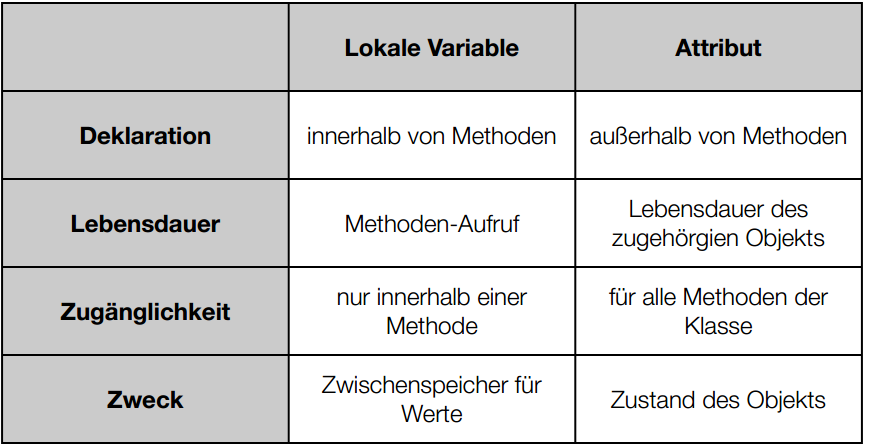
\includegraphics[width=\textwidth]{tabelle.png}
  \end{figure}
\end{frame}

\section{Sichtbarkeit}
\begin{frame}{Sichtbarkeiten}
	mit speziellen Schlüsselworten wird die Sichtbarkeit einer bestimmten Komponente (Methode, Attribut, Klasse) festgelegt.
  \begin{itemize}
    \item \textbf{kein Schlüsselwort}
    \item[] Komponente ist innerhalb des Pakets bekannt
    \pause
    \item \textbf{private}
    \item[] Komponente ist innerhalb der Klasse bekannt
    \pause
    \item \textbf{public}
    \item[] Komponente ist überall bekannt
    \pause
    \item \textbf{protected}
    \item[] Komponente ist innerhalb des Pakets und in allen Unterklassen bekannt
  \end{itemize}
\end{frame}

\begin{frame}[fragile]{Sichtbarkeiten Beispiel}
  Beispiel von vorhin mit \textbf{private}-Attributen
  \begin{lstlisting}
  public class User {   
    private String username;
    private String password;
    
    User(String username) {
      this.username = username; // Zugriff auf Instanzvariable
    }
    
    public static void main(String[] args) {
      User user = new User("Hans");
      System.out.println(user.name);
      // Was passiert?
    }
  }\end{lstlisting}
  \pause
  Lösung?
\end{frame}

\subsection{Zugriffsfunktionen}
\begin{frame}[fragile]{Zugriffsfunktionen (Getter / Setter)}
	\begin{block}{getter und setter}
    \begin{itemize}
      \item spezielle Methode zum Zugriff auf Eigenschaft eines Objekts
      \item \textbf{getter}-Methode gibt den Wert eines Attributs zurück
      \item \textbf{setter}-Methode ändert den Wert eines Attributs
    \end{itemize}
  \end{block}
   \begin{lstlisting}
  public class User {   
    private String username;
    private String password;
    
    public void setPassword(String password) { // Setter
      this.password = password;
    }
    
    public String getPassword() {  // Getter
      return this.password
    }
  }\end{lstlisting}
\end{frame}

\begin{frame}[fragile]{Zugriffsfunktionen (Getter / Setter)}
	\begin{block}{Gründe für die Verwendung von Gettern und Settern?}
    \begin{itemize}
      \item Einhaltung des Prinzips der Datenkapselung (Geheimnisprinzip)
      \pause
      \item Validierung der zu setzenden Werte
      \pause
      \item Nebenbedingungen bei get oder set
    \end{itemize}
    \end{block}
    \pause
    \begin{lstlisting}
  public class User {   
    private String password;
    
    public void setPassword(String password) { // Setter
      if ( password.length >= 6 ) {
        this.password = password;
      }
    }
    
    ...
  }\end{lstlisting}
\end{frame}


\section{Kontrollstrukturen}
\begin{frame}[fragile]{Verzweigung (\url{if})}
  \begin{block}{\url{if}-Verzweigung}
    \begin{itemize}
      \item Wertet einen Ausdruck aus und verzweigt, je nach Ergebnis
      \item der Ausdruck muss \lstinline$true$ oder \lstinline$false$ zurückliefern (\lstinline$boolean$)
      \item Ausdruck \lstinline$true$ $\Rightarrow$ nachfolgender Block wird ausgeführt
      \item optional: \lstinline$else$-Bedingung (bei \lstinline$false$ ausgeführt)
    \end{itemize}
  \end{block}
  Syntax einer \url{if-else}-Verzweigung
  \begin{lstlisting}
if (<Bedingung>) {
  <ausgefuehrt bei true>
} else {
  <ausgefuehrt bei false>
}
\end{lstlisting}   
\end{frame}

\subsection{if-Verzweigung}
\begin{frame}[fragile]{Verzweigung (\url{if})}
  Geht auch ohne geschweifte Klammern.
  \begin{lstlisting}
boolean exit = false;
if (exit)
  System.out.println("Shutting down");
  System.exit(0);
\end{lstlisting}
\textbf{Wo ist das Problem?}\\
\pause
\textbf{Lösung:} Zeile 4 wird immer ausgeführt!
\\
Desshalb immer:
\begin{itemize}
  \item \{ und \} setzen
  \item Blockinhalt einrücken
\end{itemize}
\end{frame}

\begin{frame}{Yoda-Condition}
  \begin{figure}
	\centering
  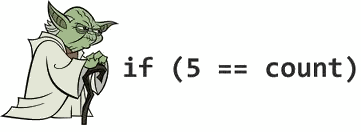
\includegraphics[width=0.7\textwidth]{yoda.png}
  \end{figure}
  \begin{itemize}
    \item Using \lstinline$if (constant = variable)$ instead of \lstinline$if (variable = constant)$
    \item Its like saying "'if blue is the sky"' or "'if tall is the man"'
  \end{itemize}
  Quelle: \href{http://www.codinghorror.com/blog/2012/07/new-programming-jargon.html}{codinghorror.com}
\end{frame}

\begin{frame}[fragile]{Mehrfachverzweigung: if-else}
  Auch möglich:
  \begin{lstlisting}
int x = 3;
if (x == 1) {
  System.out.println("x ist eins");
} else if (x == 2) {
  System.out.println("x ist zwei");
} else if (x == 3) {
  System.out.println("x ist drei");
}
  \end{lstlisting}
\end{frame}

\subsection{Mehrfachverzweigung}
\begin{frame}[fragile]{Mehrfachverzweigung: \url{switch}}
  \begin{block}{Mehrfachverzweigung: \url{switch}}
    \begin{itemize}
      \item Macht \lstinline$if-else$ Verzweigungen mit mehreren Möglichkeiten übersichtlicher
      \item Switch kann mit \lstinline$int, short, byte, char, enum$ und in Java 7 auch mit \lstinline$String$ ausgeführt werden
      \item Verzweigung anhand \lstinline$case$-Blöcke innerhalb des \lstinline$switch$-Blocks
      \item \lstinline$default$-Block wird ausgeführt, wenn keine Übereinstimmung
      \item \lstinline$break;$ als Abbruch nach jedem \lstinline$case$
    \end{itemize}
  \end{block}  
\end{frame}

\begin{frame}[fragile]{\url{switch} Beispiel}
 \begin{lstlisting}
  int month = 11;
  switch (month) {
    case 1: System.outprintln("Januar");
            break;
    case 2: System.out.println("Februar");
            break;
    ...
    case 11: System.out.println("November");
             break;
    case 12: System.out.println("Dezember");
             break;
    default: System.out.println("Monat existiert nicht!");
 }
\end{lstlisting}
\end{frame}

\begin{frame}[fragile]{\url{switch} Beispiel 2}
 \begin{lstlisting}
  int count = 1;
  switch (count) {
    case 1: System.outprintln("one");
    case 2: System.out.println("two");
    case 3: System.out.println("three");
    default: System.out.println("Counting is fun");
 }
\end{lstlisting}
\begin{center}
Welche ausgabe wird erzeugt? \newline
\pause
\parbox{10cm}{
one \newline
two \newline
three \newline
Counting is fun}
\end{center}
\end{frame}

\subsection{ternärer Operator}
\begin{frame}[fragile]{ternärer Operator}
  \begin{itemize}
    \item Besonders kompakte Darstellung einer \lstinline$if-else$-Verzweigung in einer Zeile
    \item Kann zu unleserlichem code führen!
  \end{itemize}
  Syntax:
  \begin{lstlisting}
    (<boolscher Ausdruck>) ? <true-Block> : <false-Block>;
  \end{lstlisting}
\end{frame}

\begin{frame}[fragile]{ternärer Operator}
  \begin{lstlisting}
  if (gender.equals("männlich")) {
    System.out.println ("Sehr geehrter Herr");
  } else {
    System.out.println ("Sehr geehrte Frau");
  }
  \end{lstlisting}
  Wie sieht die äquivalente Darstellung mithilfe des ternären Operators aus?\\
  \pause
  \textbf{Lösung:}
  \begin{lstlisting}
    System.out.println( "Sehr geehrte" 
         +(gender.equals("männlich") ? "r Herr" : " Frau" ));
  \end{lstlisting}
\end{frame}

\section{Aufgaben}
\subsection{Coding-Aufgaben}
\begin{frame}[fragile]{Coding-Aufgaben}
	\begin{itemize}
    \item \textbf{weekday} ist true, falls es ein Wochentag ist
    \item \textbf{vacation} ist true, falls wir in Urlaub sind
  \end{itemize}
  Vervollständige die Funktion:
  \begin{lstlisting}
    public boolean sleepIn(boolean weekday, boolean vacation) {
      // TODO
    }
  \end{lstlisting}
  \pause
  Lösung:
  \begin{lstlisting}
    public boolean sleepIn(boolean weekday, boolean vacation) {
      return !weekday || vacation;
    }
  \end{lstlisting}
\end{frame}

\begin{frame}[fragile]{Coding-Aufgaben}
	\begin{block}{Aufgabe}
    We have two monkeys, a and b, and the parameters \textbf{aSmile} and \textbf{bSmile} indicate if each is smiling. We are in trouble if they are both smiling or if neither of them is smiling. Return true if we are in trouble. 
  \end{block}
  \begin{lstlisting}
  public boolean monkeyTrouble(boolean aSmile, boolean bSmile) {
    // TODO
  }
  \end{lstlisting}
  \pause
  Lösung:
  \begin{lstlisting}
  public boolean monkeyTrouble(boolean aSmile, boolean bSmile) {
    return (aSmile && bSmile) || (!aSmile && !bSmile);
  }
  \end{lstlisting}
\end{frame}

\begin{frame}[fragile]{Coding-Aufgaben}
	\begin{block}{\textbf{substring}-Methode}
    \begin{itemize}
      \item Methode der Klasse \textbf{String}
      \item Signatur: \lstinline$String substring(int beginIndex, int endIndex)$
      \item Gibt den Teilstring zwischen \lstinline$beginIndex$ und \lstinline$endIndex$ zurück
    \end{itemize}
  \end{block}
  \pause
  Vervollständige die Funktion:
  \begin{lstlisting}
    public String notString(String str) {
  
    }\end{lstlisting}
  \textbf{Erwartetes Verhalten:}\\
  notString("`candy"') $\rightarrow$ "`not candy"'\\
  notString("`x"') $\rightarrow$ "`not x"'\\
  notString("not bad"') $\rightarrow$ "`not bad"'\\
\end{frame}

\begin{frame}[fragile]{Coding-Aufgaben}
	Lösung:
  \begin{lstlisting}
  public String notString(String str) {
    if (str.length() >= 3 && str.substring(0, 3).equals("not")) {
      return str;
    }

    return "not " + str;
  }\end{lstlisting}
\end{frame}



\section{Tutoriumsaufgabe}
\subsection{while-Schleifen}

\begin{frame}[fragile]{Tutoriumsaufgabe}
\textbf{while - Schleifen}
Aufgabe 1 (Schleifen)
Schreiben Sie in einer Klasse namens Loops die Methoden
\begin{itemize}
\item \lstinline{static boolean isPrimeWhile(int candidate)} und
\item \lstinline$static boolean isPrimeDoWhile(int candidate).$
\end{itemize}
\small{Diese sollen als Rückgabewert den Wert true haben, falls candidate eine Primzahl ist. In den
Methoden soll dabei eine while-Schleife (a)) bzw. eine do-while-Schleife (b))
verwendet werden. Beachten Sie auch die Fälle, in denen der Wert des Parameters ganz offensichtlich
keine Primzahl ist.}
\begin{itemize}
\item Schreiben Sie zusätzlich eine main-Methode
\lstinline$public static void main(String[] args),$
die alle Zahlen zwischen -1 und einer festgelegten konstanten Zahl N auf ihre Primzahl-Eigenschaft
überprüft.
\end{itemize}
\end{frame}

\begin{frame}[fragile]{Das war's für heute}
\begin{center}
Danke für eure Aufmerksamkeit!\newline
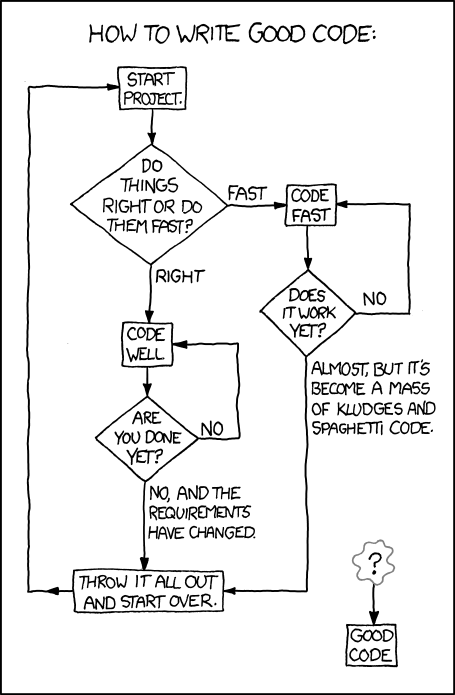
\includegraphics[width=0.6\textwidth, height= 0.8\textheight]{good_code.png}
\end{center}
\end{frame}

\subsection{Lösung Tutoriumsaufgabe}
\begin{frame}[fragile]{Lösung}
\begin{lstlisting}
static boolean tester(int n) {
		int counter = 2;
		int upTo = n/2;
		boolean valid = true;
		
		while((counter <= upTo) && (valid)) {
				if((n % counter) == 0)
				valid = false;
					counter++;
		}
		
 return valid;
}
\end{lstlisting}
\end{frame}



\appendix
\beginbackup

%\begin{frame}[allowframebreaks]{References}
%	\printbibliography
%\end{frame}

\backupend

\end{document}
